\section{Particle Identification via Bethe-Bloch}\label{ref:pid}


The energy loss of a relativistic charged particle traversing through a medium is given by the Bethe-Bloch relation:

\begin{equation}
\frac{dE}{dx} \propto \frac{1}{\beta^{2}} \frac{Z}{A} \rho \  \bigg[ \frac{1}{2} \ln \frac{2 m_{e} c^{2} \beta^{2} \gamma^{2} T_{max}}{I^{2}} - \beta^{2} - \frac{\delta \left( \beta \gamma \right) }{2} \bigg]
\end{equation}
\noindent
where $\rho$ is the density of the medium, $\frac{Z}{A}$ is the ratio of the atomic number to the atomic mass of the absorber, $\beta$ is the ratio of the particle's momentum to energy, $T_{max}$ is the maximum transfer energy from the charged particle to an electron in the medium,  $I^{2}$ is the mean excitation energy of the medium, $\frac{\delta \left( \beta \gamma \right) }{2}$ is a correction factor based on the polarization of the material, and $\gamma^{2}$ is the lorentz factor $\frac{1}{\sqrt{1-\beta^{2}}}$

\begin{figure}[h]
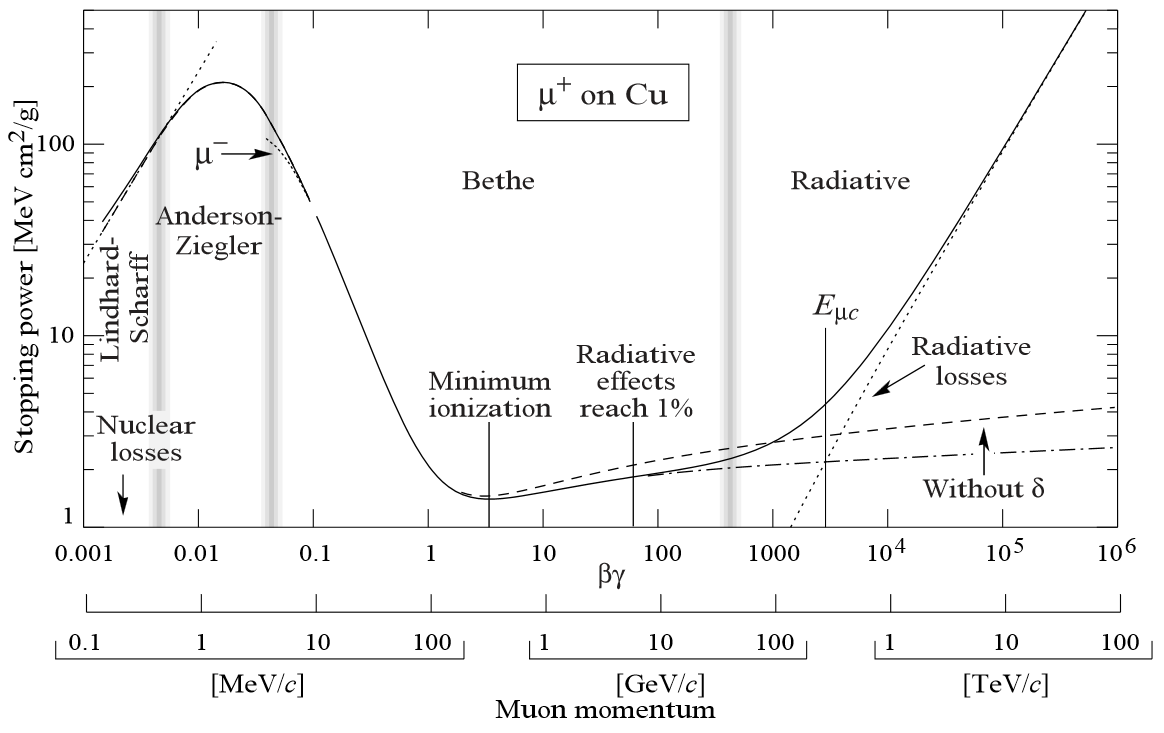
\includegraphics[width=\linewidth]{bethe}
\centering
\caption{ Energy loss of a muon traversing a copper medium between 0.1 MeV to 100 TeV \cite{Patrignani:2016xqp}.}
\label{fig:rawBB}
\end{figure}

Figure \ref{fig:rawBB} shows the Bethe-Bloch curve for a muon over a wide kinematic range.  At low energies the dominate form of energy loss is via elastic scattering, while at high energies radiation becomes the dominate energy loss mechanism. When $\beta \gamma \approx$ 3 the muon losses the least amount of energy possible and is called a minimum ionization particle(MIP).  

The ALICE ITS and TPC\footnote{See Section \ref{sec:its} and Section \ref{sec:tpc}} cannot directly measure the energy loss of a particle traversing either sub-detector.  Instead they perform PID by measuring the relative amplitudes from the sub-detectors read-out elements, pixels in the ITS and copper pads in the TPC.  The amplitudes are then fit to the Bethe-Bloch equation as seen in Figure \ref{fig:multipart-ALICE}.  Electrons weakly obey the Bethe-Bloch relationship in the kinematic ranges sensitive to the ITS and TPC and thus have a constant energy loss in both detectors.

\begin{figure}[h]
   \centering
   \subfloat[ALICE ITS(pp $\sqrt{s} = 13$ TeV )]{\label{fig:figure-a}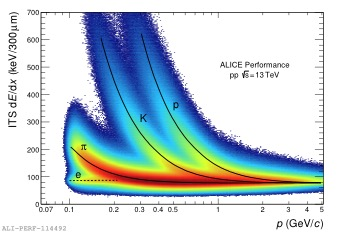
\includegraphics[width=3.0in]
     {ALICEITSPID}}
   \subfloat[ALICE TPC (PbPb $\sqrt{s_{NN}} = 5.02$ TeV )]{\label{fig:figure-b}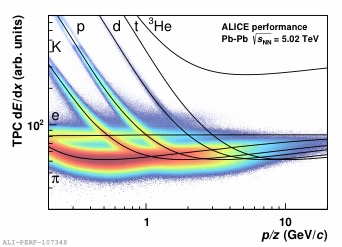
\includegraphics[width=3.0in]
     {TPC_PID2}}
   \caption{Specific energy loss for the ITS\textit{(left)} and the TPC\textit{(right)} with Bethe-Bloch fits from different particle species traversing each detector\cite{Noferini:2016lcw}.}
   \label{fig:multipart-ALICE}
\end{figure}

Figure \ref{fig:multipart-ALICE} also shows that the Bethe-Bloch curves merge above some kinematic range, 4 GeV in the ITS and 10 GeV in the TPC.  Above this kinematic range particles cannot be distinguished on a track-by-track basis, but by using statistical methods and Gaussian fits PID can be extended up to 20 GeV\cite{Abelev:2014laa}.
%\begin{figure}
%\centering
%\begin{minipage}{.5\textwidth}
  %\centering
  %\includegraphics[width=.4\linewidth]{image1}
  %\captionof{figure}{A figure}
  %\label{fig:test1}
%\end{minipage}%
%\begin{minipage}{.5\textwidth}
  %\centering
  %\includegraphics[width=.4\linewidth]{image1}
  %\captionof{figure}{Another figure}
  %\label{fig:test2}
%\end{minipage}
%\end{figure}